\chapter{El Producto de Datos}

Se cre\'o un pipeline completo que toma los par\'ametros iniciales, los cuales consisten tanto en condiciones del mundo como en los datos hist\'oricos de demanda y oferta; ejecuta el modelo de aprendizaje elegido (ya sea \textit{policy iteration} o \textit{Q-learning}; y por \'ultimo inserta los resultados en una base de datos para hacer posible consulta y an\'alisis posteriores.\\

\begin{figure}[ht]
\caption{\textit{Pipeline} del proceso}
\label{pipeline}
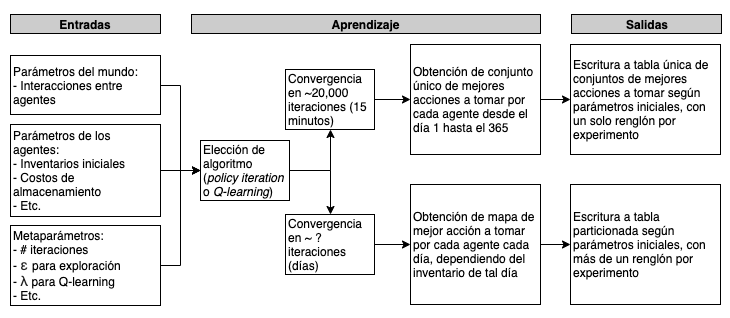
\includegraphics[width=15cm]{pipeline.PNG}
\centering
\end{figure}

Al construir la base en la cual se albergan los resultados, se adoptaron las mejores pr\'acticas para creaci\'on de bases de datos, esquemas y tablas: siguen una estructura espec\'ifica com\'unmente llamada \textit{tidy} (limpia), en la cual cada variable es una columna, cada observaci\'on una fila y cada tipo de unidad observacional es una tabla.\\

Dado que cada uno de los algoritmos de aprendizaje, \textit{policy iteration} y \textit{q-learning}, tiene requerimentos diferentes y la forma en que presenta resultados es distinta, en la base de datos se construyeron dos esquemas respectivamente, cada uno portando el nombre del algoritmo respectivo.

\section{Policy Iteration}

Es necesario crear tablas que contengan los par\'ametros necesarios: una para el mundo (tales como la demanda y oferta), otra para los agentes (tales como precios de venta, inventarios iniciales) y una \'ultima para los experimentos (los hiperpar\'ametros del algoritmo, tales como $\epsilon$ y $\lambda$). Por otro lado, dado que este m\'etodo produce una pol\'itica en forma de vector de tipo num\'erico, la manera \'optima de almacenar los resultados es en una tabla que contenga como llave el identificador (id) del experimento y el agente, y un rengl\'on por resultado.\\ 

Como llave de las tablas, se asigna el identificador (id) del experimento como el \textit{hashlib}\footnote{Las funciones de \textit{hashing} toman datos de tama\~no arbitrario y los mapean a un \textit{hash} de longitud fija.} de la concantenaci\'on de ciertos atributos de este: el sello de tiempo en el cual fue ejecutado y las \textit{policies} \'optimas de cada uno de los agentes. Esto crea un identificador \'unico y tambi\'en permite revisar que ning\'un dato haya sido modificado manualmente, en caso de que tal revisi\'on sea pertinente.\\

Se obtienen un total de 4 tablas que se relacionan de esta manera\footnote{Representaci\'on de los esquemas obtenida directamente del software }:\\

[Aqui falta el diagrama de las tablas en el esquema Policy Iteration]

% https://stackoverflow.com/questions/3223770/tools-to-generate-database-tables-diagram-with-postgresql

% https://stackoverflow.com/questions/3223770/tools-to-generate-database-tables-diagram-with-postgresql


\section{Q-Learning}

El resultado de este algoritmo es una tabla que relaciona a cada par de (estado, acci\'on) con un valor de la funci\'on Q, as\'i que no es pr\'actico utilizar el mismo formato de tabla de resultados que con \textit{policy iteration}, en el cual un rengl\'on contiene un resultado. Se crea entonces una tabla por resultado, y una tabla extra que relaciona el identificador (id) del experimento con el nombre respectivo de la tabla. El resto de la estructura del esquema es parecido al de \textit{policy iteration}, pues tambi\'en existe necesidad de relacionar los par\'ametros de cada experimento con sus resultados.\\

Debido a la estructura de la base, el n\'umero de tablas es variable, y se relacionan de esta manera:\\ 

[Aqui falta el diagrama de las tablas en el esquema Q-learning]

\section{Especificaciones t\'ecnicas}

Para el proceso se utilizaron PostgreSQL 10 y Python 3.6.5 en la distribuci\'on contenida en Anaconda, as\'i como varios paquetes de Python descritos en el archivo de requerimentos del repositorio de Github. Todos los procesos fueron ejecutados en una computadora Macbook con [] GB de RAM y [] procesadores tipo [].

[Datos faltantes]